%%%%%%%%%%%%%%%%%%%%%%%%%%%%%%%%%%%%%%%%%%%%%%%%%%%%%%%%%%%%%%%%%%%%%%%%%%%%%%%%
%% Plantilla de memoria en LaTeX para la EIF - Universidad Rey Juan Carlos
%%
%% Por Gregorio Robles <grex arroba gsyc.urjc.es>
%%     Grupo de Sistemas y Comunicaciones
%%     Escuela de Ingeniería de Fuenlabrada
%%     Universidad Rey Juan Carlos
%% (muchas ideas tomadas de Internet, colegas del GSyC, antiguos alumnos...
%%  etc. Muchas gracias a todos)
%%
%% La última versión de esta plantilla está siempre disponible en:
%%     https://github.com/gregoriorobles/plantilla-memoria
%%
%% Para obtener PDF, ejecuta en la shell:
%%   make
%% (las imágenes deben ir en PNG o JPG)

%%%%%%%%%%%%%%%%%%%%%%%%%%%%%%%%%%%%%%%%%%%%%%%%%%%%%%%%%%%%%%%%%%%%%%%%%%%%%%%%

\documentclass[a4paper, 12pt]{book}
%\usepackage[T1]{fontenc}

\usepackage[a4paper, left=2.5cm, right=2.5cm, top=3cm, bottom=3cm]{geometry}
\usepackage{times}
\usepackage[utf8]{inputenc}
\usepackage[spanish]{babel} % Comenta esta línea si tu memoria es en inglés
\usepackage{url}
%\usepackage[dvipdfm]{graphicx}
\usepackage{graphicx}
\usepackage{float}  %% H para posicionar figuras
\usepackage[nottoc, notlot, notlof, notindex]{tocbibind} %% Opciones de índice
\usepackage{latexsym}  %% Logo LaTeX

\title{Memoria del Proyecto}
\author{Nombre del autor}

\renewcommand{\baselinestretch}{1.5}  %% Interlineado

\begin{document}

\renewcommand{\refname}{Bibliografía}  %% Renombrando
\renewcommand{\appendixname}{Apéndice}


%%%%%%%%%%%%%%%%%%%%%%%%%%%%%%%%%%%%%%%%%%%%%%%%%%%%%%%%%%%%%%%%%%%%%%%%%%%%%%%%
% PORTADA

\begin{titlepage}
\begin{center}
\includegraphics[scale=0.6]{img/URJ_logo_Color_POS.png}

\vspace{1.75cm}

\LARGE
ESCUELA DE INGENIERÍA DE FUENLABRADA
\vspace{1cm}

\LARGE
INGENIERÍA EN SISTEMAS AUDIOVISUALES Y MULTIMEDIA

\vspace{1cm}
\LARGE
\textbf{TRABAJO FIN DE GRADO}

\vspace{2cm}

\Large
PLATAFORMA WEB PARA PROYECTOS DE ARQUITECTURA

\vspace{2cm}

\large
Autor : Bayas Pancho, Karol Joseth \\
Tutor : Robles Martínez, Gregorio\\
Cotutor: De Jorge Huertas, Virginia 
\vspace{1cm}

\large
Curso académico 202X/202X

\end{center}
\end{titlepage}

\newpage
\mbox{}
\thispagestyle{empty} % para que no se numere esta pagina



%%%%%%%%%%%%%%%%%%%%%%%%%%%%%%%%%%%%%%%%%%%%%%%%%%%%%%%%%%%%%%%%%%%%%%%%%%%%%%%%
%%%% Para firmar
\clearpage
\pagenumbering{gobble}
\chapter*{}

\vspace{-4cm}
\begin{center}
\LARGE
\textbf{Trabajo Fin de Grado}

\vspace{1cm}
\large
Plataforma WEB para Proyectos de Arquitectura

\vspace{1cm}
\large
\textbf{Autor :} Bayas Pancho, Karol Joseth \\
\textbf{Tutor :} Robles Martínez, Gregorio

\end{center}

\vspace{1cm}
La defensa del presente Proyecto Fin de Carrera se realizó el día \qquad$\;\,$ de \qquad\qquad\qquad\qquad \newline de 2024, siendo calificada por el siguiente tribunal:


\vspace{0.5cm}
\textbf{Presidente:}

\vspace{1.2cm}
\textbf{Secretario:}

\vspace{1.2cm}
\textbf{Vocal:}


\vspace{1.2cm}
y habiendo obtenido la siguiente calificación:

\vspace{1cm}
\textbf{Calificación:}


\vspace{1cm}
\begin{flushright}
Fuenlabrada, a \qquad$\;\,$ de \qquad\qquad\qquad\qquad de 202X
\end{flushright}

%%%%%%%%%%%%%%%%%%%%%%%%%%%%%%%%%%%%%%%%%%%%%%%%%%%%%%%%%%%%%%%%%%%%%%%%%%%%%%%%
%%%% Dedicatoria

\chapter*{}
\pagenumbering{Roman} % para comenzar la numeracion de paginas en numeros romanos
\begin{flushright}
\textit{Dedicado a \\
mi familia / mi abuelo / mi abuela}
\end{flushright}

%%%%%%%%%%%%%%%%%%%%%%%%%%%%%%%%%%%%%%%%%%%%%%%%%%%%%%%%%%%%%%%%%%%%%%%%%%%%%%%%
%%%% Agradecimientos

\chapter*{Agradecimientos}
%\addcontentsline{toc}{chapter}{Agradecimientos} % si queremos que aparezca en el índice
\markboth{AGRADECIMIENTOS}{AGRADECIMIENTOS} % encabezado 

Con la finalizacion de este proyecto doy por finalizada mi etapa universitaris por lo que antetodo me gustaria presentar la gratitud que siento hacia los profesores de la ETSI. A lo largo de estos años, su orientación y sabiduría me han guiado en mi camino académico. 
En particular, quiero expresar mi sincero agradecimiento a Gregorio Robles, quien no solo nos introdujo en el vasto mundo del desarrollo web, sino que también creyó en mí para la realización de este proyecto. Su constante disponibilidad para orientarme y su apoyo inquebrantable han sido invaluables.
No puedo dejar de mencionar el apoyo incondicional de mi familia: mis padres y hermanos. Siempre estuvieron ahí para mí, ofreciendo su aliento y amor en cada paso del camino. Sus palabras de ánimo fueron mi fuerza, y por eso les estoy eternamente agradecido.
A todos los que de alguna manera han contribuido a este trabajo, muchas gracias. Cada palabra de aliento, cada gesto de apoyo, ha sido fundamental para llegar hasta aquí. Este logro es tan suyo como mío.

%%%%%%%%%%%%%%%%%%%%%%%%%%%%%%%%%%%%%%%%%%%%%%%%%%%%%%%%%%%%%%%%%%%%%%%%%%%%%%%%
%%%% Resumen

\chapter*{Resumen}
%\addcontentsline{toc}{chapter}{Resumen} % si queremos que aparezca en el índice
\markboth{RESUMEN}{RESUMEN} % encabezado

Este proyecto representa la creación de una plataforma web dedicada a proyectos de arquitectura, 
desarrollada como parte del trabajo de fin de grado en ingeniería en sistemas audiovisuales y multimedia. 

La plataforma, construida con el framework Flask de Python, tiene como objetivo principal facilitar la 
colaboración y comunicación entre estudiantes y profesores de arquitectura. Permite a usuarios registrados, 
incluyendo alumnos y profesores, realizar diversas acciones como añadir eventos, libros y archivos. 
Además, cuenta con un administrador que gestiona la base de datos del sistema. 

La aplicación también ofrece funcionalidades para la carga y gestión de archivos, como imágenes, videos y PDFs, 
relacionados con los libros de arquitectura presentes en la plataforma. 

Diseñada para ser accesible desde cualquier navegador, la plataforma proporciona diferentes niveles 
de funcionalidad según el tipo de usuario. Este enfoque busca mejorar la experiencia educativa al 
proporcionar un medio digital para compartir información relevante y fomentar la comunicación en el
 contexto educativo de la arquitectura.

%%%%%%%%%%%%%%%%%%%%%%%%%%%%%%%%%%%%%%%%%%%%%%%%%%%%%%%%%%%%%%%%%%%%%%%%%%%%%%%%
%%%% Resumen en inglés

\chapter*{Summary}
%\addcontentsline{toc}{chapter}{Summary} % si queremos que aparezca en el índice
\markboth{SUMMARY}{SUMMARY} % encabezado

This project involves the creation of a web platform for architectural projects, developed as part
 of the final project for a degree in audiovisual and multimedia systems engineering. The main 
 objective of the platform is to facilitate collaboration and communication among architecture students 
 and professors. 
 
 Built using the Flask framework in Python, the platform allows registered users, including both students 
 and teachers, to perform various actions such as adding events, books, and files. Additionally, it features 
 an administrator who manages the system's database. 
 
 The application also provides functionalities for uploading and managing files, such as images, videos, 
 and PDFs, related to architecture books on the platform. Designed to be accessible from any internet browser, 
 the platform offers different levels of functionality depending on the type of user accessing it. 
 
 This approach aims to enhance the educational experience by providing a digital medium for sharing relevant 
 information and fostering communication in the educational context of architecture.

%%%%%%%%%%%%%%%%%%%%%%%%%%%%%%%%%%%%%%%%%%%%%%%%%%%%%%%%%%%%%%%%%%%%%%%%%%%%%%%%
%%%%%%%%%%%%%%%%%%%%%%%%%%%%%%%%%%%%%%%%%%%%%%%%%%%%%%%%%%%%%%%%%%%%%%%%%%%%%%%%
% ÍNDICES %
%%%%%%%%%%%%%%%%%%%%%%%%%%%%%%%%%%%%%%%%%%%%%%%%%%%%%%%%%%%%%%%%%%%%%%%%%%%%%%%%

% Las buenas noticias es que los índices se generan automáticamente.
% Lo único que tienes que hacer es elegir cuáles quieren que se generen,
% y comentar/descomentar esa instrucción de LaTeX.

%%%% Índice de contenidos
\tableofcontents 
%%%% Índice de figuras
\cleardoublepage
%\addcontentsline{toc}{chapter}{Lista de figuras} % para que aparezca en el indice de contenidos
\listoffigures % indice de figuras
%%%% Índice de tablas
%\cleardoublepage
%\addcontentsline{toc}{chapter}{Lista de tablas} % para que aparezca en el indice de contenidos
%\listoftables % indice de tablas


%%%%%%%%%%%%%%%%%%%%%%%%%%%%%%%%%%%%%%%%%%%%%%%%%%%%%%%%%%%%%%%%%%%%%%%%%%%%%%%%
%%%%%%%%%%%%%%%%%%%%%%%%%%%%%%%%%%%%%%%%%%%%%%%%%%%%%%%%%%%%%%%%%%%%%%%%%%%%%%%%
% INTRODUCCIÓN %
%%%%%%%%%%%%%%%%%%%%%%%%%%%%%%%%%%%%%%%%%%%%%%%%%%%%%%%%%%%%%%%%%%%%%%%%%%%%%%%%

\cleardoublepage
\chapter{Introducción}
\label{sec:intro} % etiqueta para poder referenciar luego en el texto con ~\ref{sec:intro}
\pagenumbering{arabic} % para empezar la numeración de página con números

En el ámbito de la educación arquitectónica, la necesidad de una colaboración eficiente y una 
comunicación fluida se ha vuelto cada vez más crucial. Este proyecto aborda esta necesidad al introducir 
una plataforma web sofisticada diseñada para estudiantes y profesores en el campo de la arquitectura. 

Desarrollada como culminación del proyecto final para obtener un título en ingeniería de sistemas audiovisuales 
y multimedia, la plataforma sirve como un centro centralizado para compartir información relevante y facilitar 
la comunicación sobre eventos en curso a lo largo de los cursos académicos.

\section{Motivación}
\label{sec:seccion}


En el trasfondo de la educación arquitectónica, me impulsa la firme convicción de que la tecnología puede desempeñar un papel transformador al mejorar la colaboración y la comunicación entre estudiantes y profesores. Inspirado por mis tutores Virginia y Gregorio en el deseo de superar las barreras existentes en la interacción educativa, he decidido emprender el desarrollo de esta plataforma web.

La motivación central detrás de esta iniciativa es la necesidad de proporcionar a la comunidad educativa de arquitectura una herramienta digital que simplifique y enriquezca su experiencia de aprendizaje. Observando las limitaciones en la comunicación y el intercambio de información, he visualizado esta plataforma como un espacio virtual donde la colaboración se vuelve intuitiva y donde la información relevante fluye de manera efectiva.

Con el objetivo de fomentar la participación activa, la plataforma busca ir más allá de ser simplemente un repositorio de datos. Pretende ser un medio dinámico donde los estudiantes pueden compartir ideas, los profesores pueden proporcionar orientación y todos pueden estar al tanto de los eventos educativos cruciales. La creación de esta plataforma no solo es un ejercicio técnico, sino una contribución tangible a la mejora de la calidad educativa en el ámbito de la arquitectura.

Creo firmemente que, al proporcionar un entorno digital eficiente y fácil de usar, esta plataforma puede marcar la diferencia al facilitar la colaboración, fomentar la comunicación y, en última instancia, elevar el estándar de la educación arquitectónica. Esta motivación arraigada en la mejora continua y la innovación tecnológica impulsa mi dedicación a la creación de esta herramienta que aspira a enriquecer la experiencia educativa para estudiantes y profesores por igual.
\section{Objetivos e hipótesis de investigación}
\label{sec:seccion}

\subsection{Objetivos de Investigación}
\label{subsec:Objetivos de Investigación}

\begin{itemize}
  \item Facilitar la Colaboración: Crear un entorno digital que promueva la colaboración entre estudiantes y profesores de arquitectura, facilitando el intercambio de información y recursos educativos.
  \item Centralizar Recursos: Desarrollar una plataforma que sirva como repositorio central para libros, archivos y otros recursos relacionados con la arquitectura, mejorando el acceso y la gestión de la información educativa.
  \item Mejorar la Comunicación: Implementar herramientas de comunicación efectiva, como la organización de eventos y foros, para fomentar la interacción activa y el intercambio de ideas entre los usuarios.
  \item Optimizar la Experiencia del Usuario: Diseñar una interfaz intuitiva y fácil de usar que se adapte a las necesidades específicas de los estudiantes y profesores de arquitectura, mejorando la experiencia de navegación y participación.
\end{itemize}

\subsection{Hipótesis de Investigación}
\label{subsec:Hipótesis de Investigación}

\begin{itemize}
  \item Mayor Colaboración con la Plataforma: Se espera que la implementación de la plataforma web aumente la colaboración entre estudiantes y profesores, proporcionando un espacio digital propicio para compartir conocimientos y experiencias.
  \item Eficiencia en la Gestión de Recursos: La centralización de recursos, como libros y archivos, en la plataforma resultará en una gestión más eficiente y accesible de los materiales educativos, beneficiando tanto a estudiantes como a profesores.
  \item Mejora en la Comunicación: La introducción de herramientas de comunicación, como eventos y foros, contribuirá a una comunicación más efectiva entre los usuarios, fomentando la participación activa y la discusión de temas relevantes.
  \item Aumento de la Participación: La optimización de la experiencia del usuario en la plataforma generará un aumento en la participación, ya que los usuarios encontrarán la interfaz intuitiva y amigable, facilitando su interacción con la plataforma.
\end{itemize}

{\footnotesize
\begin{center}
\begin{verbatim}
proyecto_arquitectura/
|-- static/
|   |-- archivos/
|   |   |-- imagenes/
|   |   |-- videos/
|   |   |-- pdf/
|   |-- css/
|   |-- js/
|-- templates/
|   |-- admin/
|   |   |-- index.html
|   |   |-- login.html
|   |   |-- registro.html
|   |   |-- ...
|   |-- sitio/
|       |-- books.html
|       |-- calendar.html
|       |-- ...
|-- sitio_routes.py
|-- admin_routes.py
|-- decorators.py
|-- config.py
|-- app.py
|-- requirements.txt
\end{verbatim}
\end{center}
}

\section{Estructura de la memoria}
\label{sec:seccion}

A continuación, se presenta una descripción de la estructura de la memoria, 
detallando el contenido de cada uno de los capítulos para proporcionar 
una guía organizada del trabajo de fin de grado:

\begin{itemize}
  \item \textbf{Capítulo 1:} Introducción \\
  En este capítulo, se presenta el contexto del trabajo, se define el problema de 
  investigación y se destacan los objetivos del estudio. Además, se ofrece una breve 
  descripción de la metodología utilizada y se justifica la relevancia del tema.
  \item \textbf{Capítulo 2:} Objetivos del Proyecto \\
  En este capítulo se proporciona información detallada sobre el diseño, las 
  características y los usos de cada una de las tecnologías usadas en el proyecto. 

  \item \textbf{Capítulo 3:} Tecnologías Utilizadas \\
  En este capítulo se proporciona información detallada sobre el diseño, las 
  características y los usos de cada una de las tecnologías usadas en el proyecto.

  \item \textbf{Capítulo 4:} Funcionamiento de la Aplicación \\
  En este capítulo, se entra en detalle en el funcionamiento de la aplicación.

  \item \textbf{Capítulo 5:} Experimentos y Pruebas \\
  Se presentan los diferentes experimentos realizados y se prueba el correcto funcionamiento de la aplicación.

  \item \textbf{Capítulo 6:} Resultados Obtenidos \\
  En este capítulo, se explican los resultados obtenidos al poner a prueba varios aspectos de la aplicación.

  \item \textbf{Capítulo 7:} Conclusiones \\
  Se indican los resultados conseguidos y la solución a los objetivos no conseguidos.
\end{itemize}


%%%%%%%%%%%%%%%%%%%%%%%%%%%%%%%%%%%%%%%%%%%%%%%%%%%%%%%%%%%%%%%%%%%%%%%%%%%%%%%%
%%%%%%%%%%%%%%%%%%%%%%%%%%%%%%%%%%%%%%%%%%%%%%%%%%%%%%%%%%%%%%%%%%%%%%%%%%%%%%%%
% OBJETIVOS %
%%%%%%%%%%%%%%%%%%%%%%%%%%%%%%%%%%%%%%%%%%%%%%%%%%%%%%%%%%%%%%%%%%%%%%%%%%%%%%%%

\cleardoublepage % empezamos en página impar
\chapter{Objetivos} % título del capítulo (se muestra)
\label{chap:objetivos} % identificador del capítulo (no se muestra, es para poder referenciarlo)

\section{Objetivo general} % título de sección (se muestra)
\label{sec:objetivo-general} % identificador de sección (no se muestra, es para poder referenciarla)
El propósito de este proyecto es crear un sistema de administración destinado a gestionar libros, documentos y eventos. 
Su objetivo principal es mejorar la experiencia de los usuarios al facilitar el acceso a la información a través de una 
interfaz intuitiva. Para garantizar la seguridad de la plataforma, se implementarán funcionalidades como inicio de sesión 
y restablecimiento de contraseña.

En esta plataforma, nos centramos en la interacción de los usuarios para la gestión de eventos y la administración de libros. 
También hemos integrado herramientas administrativas que facilitarán a los usuarios interactuar de manera eficiente y efectiva. 
Queremos que la experiencia sea lo más amigable posible para todos los que utilicen este sistema.
\section{Objetivos específicos}
\label{sec:objetivos-especificos}
\begin{enumerate}
  \item \textbf{Desarrollar vistas de administración:} Crear vistas administrativas para la gestión de libros, eventos y usuarios.
  \item \textbf{Sistema de autenticación:} Desarrollar un sistema de autenticación para permitir el acceso seguro a las funcionalidades administrativas.
  \item \textbf{Diseñar páginas de visualización:} Diseñar páginas de visualización de libros, eventos y comentarios para todos los usuarios.
  \item \textbf{Integrar un sistema de comentarios:} Integrar un sistema de comentarios para permitir a los usuarios expresar sus opiniones sobre los libros.
  \item \textbf{Gestión de eventos:} Implementar la gestión de eventos, permitiendo la visualización y edición de ellos.
  \item \textbf{Administrar libros:} Desarrollar funciones para agregar, editar y eliminar libros ademas de asociarlos con autores.
  \item \textbf{Herramientas administrativas:} Implementar herramientas administrativas para la gestión de usuarios, roles y permisos.
  \item \textbf{Optimizar seguridad:} Mejorar la seguridad de las contraseñas mediante el uso de técnicas seguras de almacenamiento y recuperación.
  \item \textbf{Restricciones de acceso:} Aplicar restricciones de acceso basadas en roles para controlar qué usuarios pueden acceder a determinadas funcionalidades.
  \item \textbf{Integridad de los datos:} Implementar medidas para garantizar la integridad de los datos, evitando inconsistencias y errores en la base de datos.
\end{enumerate}

\section{Planificación temporal}
\label{sec:planificacion-temporal}

A finales de julio del año pasado, inicié mi proyecto de fin de grado. Todo comenzó en julio de 2023 cuando el profesor 
Gregorio Robles Martínez me sugirió la idea del proyecto que he llevado a cabo.

Durante los meses de julio y agosto, comencé a reunirme con Virginia, mi cotutora del Trabajo de Fin de Grado (TFG), 
y juntos empezamos a planificar las partes básicas que quería reflejar en el sitio web. Luego, realicé un estudio de 
diversas páginas que ella me proporcionó, de las cuales obtuve algunas ideas para implementar en el proyecto.

De agosto a octubre, me sumergí en la implementación de la página web, siguiendo ciertos requisitos como una vista para 
usuarios registrados y otra pública. La vista de usuario se detalló en cada tutoría, abordando aspectos como la implementación 
de diferentes permisos, la admisión de usuarios y la recuperación de contraseñas.

En los meses de noviembre y diciembre, se llevó a cabo la incorporación del calendario y la vista de libros, con comentarios 
exclusivamente para usuarios registrados. Fue en diciembre cuando comencé la redacción de la memoria del proyecto.
\begin{figure}
  \centering
  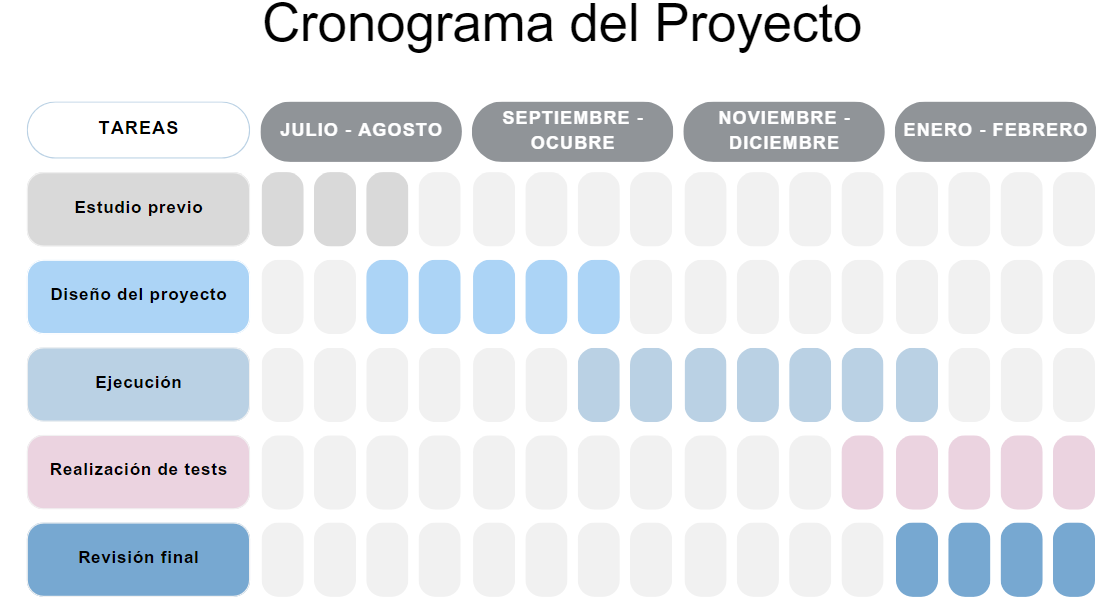
\includegraphics[width=15cm, keepaspectratio]{img/gann.png}
  \caption{Diagrama de Gantt}
  \label{fig:arquitectura}
\end{figure}


%%%%%%%%%%%%%%%%%%%%%%%%%%%%%%%%%%%%%%%%%%%%%%%%%%%%%%%%%%%%%%%%%%%%%%%%%%%%%%%%
%%%%%%%%%%%%%%%%%%%%%%%%%%%%%%%%%%%%%%%%%%%%%%%%%%%%%%%%%%%%%%%%%%%%%%%%%%%%%%%%
% ESTADO DEL ARTE %
%%%%%%%%%%%%%%%%%%%%%%%%%%%%%%%%%%%%%%%%%%%%%%%%%%%%%%%%%%%%%%%%%%%%%%%%%%%%%%%%

\cleardoublepage
\chapter{Estado del arte}
\label{chap:estado}

En este capítulo se mostraran las herramientas y liberías usadas en el Trabajo de Fin de Grado. Esto nos 
dara una visión de las tecnologias utilizadas a lo largo del proyecto.

\section{Tecnologías y Herrmientas}
\label{sec:tecnologías y herramientas}

\subsection{Python}
\label{subsec:Python}
Python fue creado por Guido van Rossum a finales de los 80 y principios de los 90 en los Países Bajos. 
Van Rossum diseñó el lenguaje con un enfoque en la legibilidad del código y la productividad del programador. 
Su nombre está inspirado en los Monty Python, que era un grupo de comedia británico que el creador admiraba. 

La primera versión, Python 0.9.0, fue lanzada en 1991, y desde entonces ha experimentado un crecimiento significativo, 
convirtiéndose en uno de los lenguajes de programación más populares y utilizados en la actualidad.

Python se destaca por su sintaxis simple, clara y precisa, la cual facilita la escritura de un código limpio y comprensible. 
Además, cuenta con una amplia gama de bibliotecas estándar las cuales abarcan desde la manipulación de datos hasta el desarrollo web, 
lo que acelera el proceso de desarrollo al proporcionar módulos y paquetes preexistentes. Esta capacidad de adaptación y su compatibilidad 
con diversos paradigmas de programación, como la orientación a objetos y la funcional, han contribuido a su éxito en una variedad de aplicaciones, 
desde desarrollo de software hasta análisis de datos y machine learning.

\subsection{GitHub}
\label{subsec:github}
GitHub\footnote{\url{https://github.com/}} es un servicio basado en la nube que aloja un sistema de control de versiones (VCS) conocido como Git. Este sistema posibilita a los desarrolladores colaborar y efectuar cambios en proyectos compartidos mientras mantienen un seguimiento detallado de su progreso. Funciona como una plataforma web de desarrollo colaborativo de software, facilitando la colaboración y almacenamiento de proyectos, ya sean de código abierto o cerrado.

En GitHub, los usuarios pueden crear y unirse a proyectos, permitiéndoles compartir ideas, discutir posibles soluciones y colaborar para mejorar los proyectos existentes. La principal ventaja de GitHub es la capacidad de trabajar en un proyecto desde cualquier lugar y en cualquier momento, ya que registra el desarrollo de los proyectos de forma remota en la nube, eliminando la necesidad de una infraestructura de hardware específica.

La función principal de GitHub se centra en ofrecer a los desarrolladores herramientas esenciales, como bibliotecas y funciones para la gestión de versiones del software, manejo de problemas, revisión de código, entre otras. La plataforma integra la funcionalidad de Git, un sistema de control de versiones distribuido que registra un historial completo de cambios, permitiendo revisar y deshacer modificaciones en el código a lo largo del tiempo. Esta característica posibilita la colaboración de varios desarrolladores en un mismo proyecto.

\subsection{PHPMyAdmin}
\label{subsec:phpmyadmin}

PHPMyAdmin es una herramienta escrita en PHP diseñada para facilitar la administración de bases de datos MySQL a través de páginas web, 
utilizando un navegador. Su funcionalidad abarca la creación y eliminación de bases de datos, así como la capacidad de crear, modificar 
y eliminar tablas. Permite realizar operaciones como borrar, editar y añadir campos, ejecutar sentencias SQL, administrar claves en campos, 
gestionar privilegios y exportar datos en diversos formatos. Con soporte para 72 idiomas, esta herramienta está disponible bajo la licencia 
GPL Versión 2.

Desde su inicio en 1998, PHPMyAdmin ha sido altamente valorado en la comunidad de descargas de SourceForge.net, destacándose como la 
descarga del mes de diciembre de 2002. A lo largo de su desarrollo, ha evolucionado tecnológicamente, adaptándose a las máquinas con 
Servidores Webs y Soporte de PHP y MySQL.

\subsection{JavaScript}
\label{subsec:JavaScript}
JavaScript\footnote{\url{https://developer.mozilla.org/es/docs/Web/JavaScript/Guide}} es un lenguaje de programación de alto nivel, interpretado y orientado a objetos. Es principalmente conocido por su capacidad para agregar interactividad y dinamismo a las páginas web. 

Algunos puntos clave sobre JavaScript:

\begin{enumerate}
  \item \textbf{Lenguaje del lado del cliente:} JavaScript se ejecuta en el navegador del usuario, lo que lo convierte en un lenguaje de programación del lado del cliente. 
  Esto significa que es procesado por el navegador web y puede interactuar con el contenido de la página, el DOM (Document Object Model) y otros elementos del navegador.
  \item \textbf{Interactividad en el navegador:} JavaScript se utiliza comúnmente para agregar interactividad a las páginas web. Puede manipular el contenido de la página, 
  responder a eventos del usuario (como clics y teclas), realizar validaciones de formularios y más.
  \item \textbf{Asíncrono y callbacks:} Se trata de un lenguaje asincrónico por naturaleza, lo que significa que puede realizar tareas sin bloquear la ejecución del código. 
  Esto se logra a través de callbacks y promesas, permitiendo operaciones como la carga de datos o la actualización del DOM sin detener la ejecución del resto del código.
  \item \textbf{DOM Manipulation:} Es fundamental para la manipulación del DOM, que es la representación en memoria de la estructura de un documento HTML. 
  Puede agregar, eliminar o modificar elementos en el DOM dinámicamente.
  \item \textbf{Eventos:} JavaScript permite manejar eventos del usuario, como clics, teclas presionadas, desplazamientos, etc. Esto facilita la creación de aplicaciones 
  web interactivas y receptivas.
  \item \textbf{Ajax:} Se utiliza comúnmente en combinación con tecnologías como XMLHttpRequest o la interfaz Fetch para realizar solicitudes asíncronas al servidor y actualizar partes específicas de la página sin necesidad de recargarla por completo.
  \item \textbf{Frameworks y bibliotecas:} Existen numerosos frameworks y bibliotecas de JavaScript, como React, Angular y Vue.js, que facilitan el desarrollo de aplicaciones web complejas 
  mediante el uso de patrones y componentes predefinidos.
  \item \textbf{ECMAScript:} Sigue las especificaciones definidas por ECMAScript, que establece las reglas y características del lenguaje. Las nuevas versiones de ECMAScript introducen mejoras 
  y características adicionales, como las arrow functions, async/await, clases, y más.
  \item \textbf{Pluriparadigmático:} Es un lenguaje de programación pluriparadigmático, lo que significa que admite varios estilos de programación, incluyendo programación orientada a objetos, funcional y procedural.
\end{enumerate}

\section{Liberías}
\label{sec:Librerias}

Descripción de las tecnologías utilizadas en el proyecto. 

\subsection{Flask}
\label{subsec:flask}
Flask es un framework de web ligero y flexible para construir aplicaciones web en Python. Desarrollado por Armin Ronacher, 
Flask se destaca por su simplicidad y su enfoque minimalista, permitiendo a los desarrolladores elegir las herramientas y 
bibliotecas que mejor se adapten a sus necesidades.

Características clave de Flask:
\begin{enumerate}
  \item \textbf{Simplicidad:} Flask sigue el principio de "hacer lo simple", proporcionando solo lo esencial para construir aplicaciones web. Su estructura modular permite a los desarrolladores agregar componentes según sea necesario.
  \item \textbf{Microframework:} Flask es considerado un microframework, lo que significa que proporciona solo las características esenciales para construir aplicaciones web. Esto ofrece flexibilidad para elegir y agregar extensiones y bibliotecas según las necesidades del proyecto.
  \item \textbf{Extensibilidad:} A pesar de ser liviano, Flask es altamente extensible. Ofrece una amplia gama de extensiones para agregar funcionalidades específicas, como la autenticación, manejo de formularios, ORM (Object-Relational Mapping), entre otras.
  \item \textbf{Jinja2 como motor de plantillas:} Flask utiliza Jinja2 como su motor de plantillas, lo que permite a los desarrolladores generar contenido dinámico de manera sencilla y legible.
  \item \textbf{Desarrollo rápido:} Flask facilita el desarrollo rápido de aplicaciones web al proporcionar un conjunto de herramientas básicas y una estructura simple. Esto lo convierte en una excelente opción para prototipos y proyectos pequeños, así como para aplicaciones web más complejas.
  \item \textbf{Compatibilidad con HTTP:} Flask tiene una excelente compatibilidad con el protocolo HTTP, facilitando la manipulación de solicitudes y respuestas HTTP.
  \item \textbf{Servidor de desarrollo incorporado:} Flask incluye un servidor de desarrollo incorporado, lo que facilita probar y depurar aplicaciones durante el desarrollo sin necesidad de configuraciones adicionales.
  \item \textbf{Comunidad activa:} Flask cuenta con una comunidad activa de desarrolladores y una documentación bien estructurada, lo que facilita aprender y resolver problemas.
\end{enumerate}

\subsection{MySQL}
\label{subsec:mysql}
MySQL es un sistema de gestión de bases de datos relacional (RDBMS) de código abierto que utiliza el lenguaje de consulta estructurado (SQL) para gestionar y manipular datos. Fue desarrollado originalmente por MySQL AB, que luego fue adquirida por Sun Microsystems y, finalmente, por Oracle Corporation.

Aquí hay algunas características clave de MySQL:
\begin{enumerate}
  \item \textbf{Relacional:} MySQL sigue el modelo relacional, lo que significa que organiza los datos en tablas con filas y columnas. Utiliza claves primarias y foráneas para establecer relaciones entre tablas.
  \item \textbf{SQL:} MySQL utiliza SQL como lenguaje para realizar consultas y manipular datos. Es compatible con las funciones estándar de SQL, pero también incluye extensiones y características propias.
  \item \textbf{Escalabilidad:} MySQL es conocido por su capacidad de escalar desde aplicaciones pequeñas hasta sistemas empresariales de gran envergadura. Ofrece opciones para replicación, particionamiento y clustering.
  \item \textbf{Soporte para Transacciones:} MySQL es compatible con transacciones, lo que garantiza la consistencia de los datos incluso en entornos con múltiples operaciones concurrentes. Utiliza el concepto de COMMIT y ROLLBACK para confirmar o deshacer transacciones.
  \item \textbf{Multiplataforma:} MySQL es compatible con varias plataformas, incluyendo sistemas operativos como Linux, Windows y macOS. Esto facilita la portabilidad de las aplicaciones desarrolladas con MySQL.
  \item \textbf{Almacenamiento de Datos:} MySQL ofrece diferentes motores de almacenamiento, cada uno con sus propias características. InnoDB es uno de los motores más populares y es conocido por su soporte de transacciones ACID.
  \item \textbf{Comunidad Activa:} MySQL cuenta con una amplia comunidad de usuarios y desarrolladores. Además, existe una versión de código abierto llamada MySQL Community Edition, así como una versión comercial con características adicionales denominada MySQL Enterprise Edition.
  \item \textbf{Herramientas y Utilidades:} MySQL proporciona varias herramientas y utilidades para administrar y monitorear bases de datos. Entre ellas se incluyen MySQL Workbench para diseño y administración visual, así como utilidades de línea de comandos como mysqldump y mysqladmin.
\end{enumerate}
MySQL es ampliamente utilizado en el desarrollo web y en una variedad de aplicaciones, desde sitios web pequeños hasta aplicaciones empresariales complejas. Su popularidad se debe a su rendimiento confiable, su naturaleza de código abierto y su robusta comunidad de usuarios.

\subsection{Bootstrap}
\label{subsec:bootstrap}
Bootstrap es un popular framework de desarrollo frontend que facilita la creación de interfaces de usuario atractivas y responsivas para aplicaciones web. Fue creado por Twitter y está basado en HTML, CSS y JavaScript. Aquí hay algunas características clave de Bootstrap:

\begin{enumerate}
  \item \textbf{Diseño Responsivo} Bootstrap se destaca por su diseño responsivo, lo que significa que las aplicaciones web construidas con Bootstrap se adaptan de manera automática y elegante a diferentes tamaños de pantalla, ya sea en dispositivos móviles, tabletas o computadoras de escritorio.
  \item \textbf{Grid System:} Bootstrap utiliza un sistema de rejilla (grid system) para organizar el diseño de la página en filas y columnas. Esto facilita la creación de diseños flexibles y adaptables.
  \item \textbf{Componentes Reutilizables:} Bootstrap ofrece una amplia variedad de componentes predefinidos, como botones, formularios, navegación, alertas y más. Estos componentes son fáciles de usar y pueden personalizarse según las necesidades del proyecto.
  \item \textbf{Tipografía y Estilos:} Bootstrap incluye estilos predeterminados para la tipografía, lo que garantiza una apariencia consistente en toda la aplicación. También proporciona clases CSS para estilizar elementos comunes de manera rápida.
  \item \textbf{JavaScript Incorporado:} Bootstrap incluye funcionalidades interactivas y dinámicas gracias al uso de JavaScript. Esto incluye componentes como modales, carruseles, desplegables y más.
  \item \textbf{Personalización:} Aunque Bootstrap ofrece un conjunto completo de estilos y componentes, es altamente personalizable. Los desarrolladores pueden ajustar el aspecto y la sensación de sus aplicaciones modificando variables en el código fuente o utilizando temas personalizados.
  \item \textbf{Documentación Detallada:} Bootstrap cuenta con una documentación exhaustiva y fácil de entender. Esta documentación proporciona ejemplos de código y guías que ayudan a los desarrolladores a utilizar eficazmente las características de Bootstrap.
  \item \textbf{Comunidad Activa:} Bootstrap cuenta con una amplia comunidad de desarrolladores y diseñadores, lo que facilita la obtención de ayuda, recursos adicionales y contribuciones a la mejora continua del framework.
\end{enumerate}
Con dos o tres párrafos por cada tecnología, vale. 
Se supone que aquí viene todo lo que no has hecho tú.

Puedes citar libros, como el de Bonabeau et al., sobre procesos estigmérgicos~\cite{bonabeau:_swarm}. 
Me encantan los procesos estigmérgicos.
Deberías leer más sobre ellos.
Pero quizás no ahora, que tenemos que terminar la memoria para sacarnos por fin el título.
Nota que el \~ \ añade un espacio en blanco, pero no deja que exista un salto de línea. 
Imprescindible ponerlo para las citas.

Citar es importantísimo en textos científico-técnicos. 
Porque no partimos de cero.
Es más, partir de cero es de tontos; lo suyo es aprovecharse de lo ya existente para construir encima y hacer cosas más sofisticadas.
¿Dónde puedo encontrar textos científicos que referenciar?
Un buen sitio es Google Scholar\footnote{\url{http://scholar.google.com}}.
Por ejemplo, si buscas por ``stigmergy libre software'' para encontrar trabajo sobre software libre y el concepto de \emph{estigmergia} (¿te he comentado que me gusta el concepto de estigmergia ya?), encontrarás un artículo que escribí hace tiempo cuyo título es ``Self-organized development in libre software: a model based on the stigmergy concept''.
Si pulsas sobre las comillas dobles (entre la estrella y el ``citado por ...'', justo debajo del extracto del resumen del artículo, te saldrá una ventana emergente con cómo citar.
Abajo a la derecha, aparece un enlace BibTeX.
Púlsalo y encontrarás la referencia en formato BibTeX, tal que así:

{\footnotesize
\begin{verbatim}
@inproceedings{robles2005self,
  title={Self-organized development in libre software:
         a model based on the stigmergy concept},
  author={Robles, Gregorio and Merelo, Juan Juli\'an 
          and Gonz\'alez-Barahona, Jes\'us M.},
  booktitle={ProSim'05},
  year={2005}
}
\end{verbatim}
}

Copia el texto en BibTeX y pégalo en el fichero \texttt{memoria.bib}, que es donde están las referencias bibliográficas.
Para incluir la referencia en el texto de la memoria, deberás citarlo, como hemos hecho antes con~\cite{bonabeau:_swarm}, lo que pasa es que en vez de el identificador de la cita anterior (bonabeau:\_swarm), tendrás que poner el nuevo (robles2005self).
Compila el fichero \texttt{memoria.tex} (\texttt{pdflatex memoria.tex}), añade la bibliografía (\texttt{bibtex memoria.aux}) y vuelve a compilar \texttt{memoria.tex} (\texttt{pdflatex memoria.tex})\ldots y \emph{voilà} ¡tenemos una nueva cita~\cite{robles2005self}!

También existe la posibilidad de poner notas al pie de página, por ejemplo, una para indicarte que visite la página del GSyC\footnote{\url{http://gsyc.es}}.



\section{Sección 1} 
\label{sec:seccion1}

Hemos hablado de cómo incluir figuras.
Pero no hemos dicho nada de tablas.
A mí me gustan las tablas.
Mucho.
Aquí un ejemplo de tabla, la Tabla~\ref{tab:ejemplo} (siento ser pesado, pero nota cómo he puesto la referencia).

\begin{table}
 \begin{center}
  \begin{tabular}{ | l | c | r |} % tenemos tres colummnas, la primera alineada a la izquierda (l), la segunda al centro (c) y la tercera a la derecha (r). El | indica que entre las columnas habrá una línea separadora.
    \hline
    Uno & 2 & 3 \\ \hline % el hline nos da una línea vertical
    Cuatro & 5 & 6 \\ \hline
    Siete & 8 & 9 \\
    \hline
  \end{tabular}
  \caption{Ejemplo de tabla. Aquí viene una pequeña descripción (el \emph{caption}, el pie de tabla/figura) del contenido de la tabla. Si la tabla no es autoexplicativa, siempre viene bien aclararla aquí.}
  \label{tab:ejemplo}
 \end{center}
\end{table}

Hay un sitio en Internet donde puedes diseñar las tablas fácilmente y luego hacer un corta y pega del resultado en tu editor.
Puedes probarlo en \url{https://www.tablesgenerator.com/}.



%%%%%%%%%%%%%%%%%%%%%%%%%%%%%%%%%%%%%%%%%%%%%%%%%%%%%%%%%%%%%%%%%%%%%%%%%%%%%%%%
%%%%%%%%%%%%%%%%%%%%%%%%%%%%%%%%%%%%%%%%%%%%%%%%%%%%%%%%%%%%%%%%%%%%%%%%%%%%%%%%
% DISEÑO E IMPLEMENTACIÓN %
%%%%%%%%%%%%%%%%%%%%%%%%%%%%%%%%%%%%%%%%%%%%%%%%%%%%%%%%%%%%%%%%%%%%%%%%%%%%%%%%

\cleardoublepage
\chapter{Diseño e implementación}
\label{sec:diseno}

A continuación, se expondrán con detalle los métodos y herramientas empleados en la ejecución del proyecto, 
ofreciendo una perspectiva minuciosa sobre el desarrollo de la iniciativa que tiene como finalidad la creación 
de una página web para el almacenamiento de toda la documentación relevante. Este capítulo ahonda en las diversas 
etapas del proyecto, detallando las decisiones adoptadas y las justificaciones vinculadas a las metodologías seleccionadas. 
Asimismo, se expone el diseño e implementación del proyecto con la intención de proporcionar a otros la capacidad de 
contribuir, adaptar o ampliar el sistema. Esta sección brinda una visión completa de cómo se estructuró y llevó a cabo 
el proyecto, abarcando las distintas fases de su creación.



\section{Arquitectura general} 
\label{sec:arquitectura}


En la Figura 4.1 se muestra un esquema general de la estructura de la página web. En esta página, 
se puede acceder tanto como usuario registrado o como visitante. La diferencia principal radica en 
los privilegios para realizar ciertas acciones.

Cuando accedes como visitante, tienes acceso a la vista de la página, lo que significa que puedes 
ver el contenido que se encuentra publicado. Sin embargo, no puedes comentar, subir contenido nuevo 
ni dejar comentarios en las publicaciones existentes. Estas funciones están reservadas para los usuarios 
registrados, quienes tienen permisos adicionales para interactuar con la página.
\begin{figure}
  \centering
  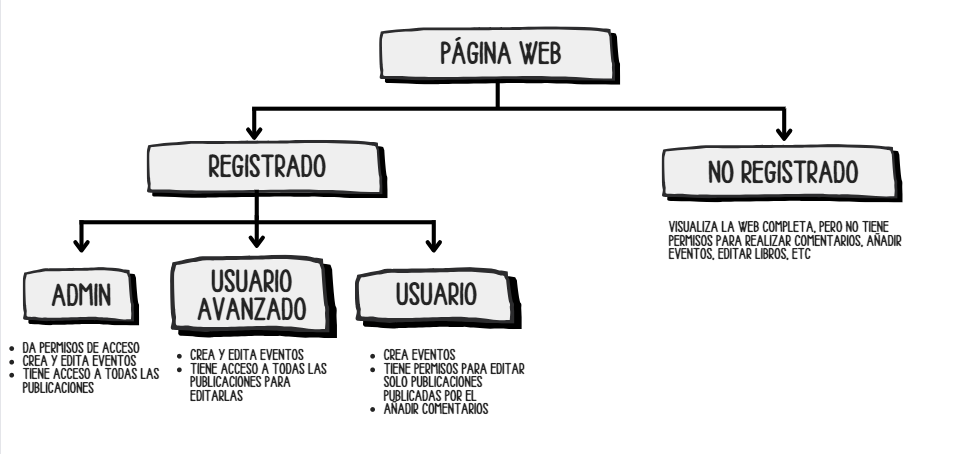
\includegraphics[width=9cm, keepaspectratio]{img/esquema.png}
  \caption{Estructura página web}
  \label{fig:arquitectura}
\end{figure}

La pagina esta diseñada con el framework de Flask, utiliza una base de datos de xampp el cual esta
Por ejemplo, puedes verlo en la figura~\ref{fig:arquitectura}.
\LaTeX \ pone las figuras donde mejor cuadran. 
Y eso quiere decir que quizás no lo haga donde lo hemos puesto\ldots 
Eso no es malo.
A veces queda un poco raro, pero es la filosofía de \LaTeX: tú al contenido, que yo me encargo de la maquetación.


 
Recuerda que toda figura que añadas a tu memoria debe ser explicada.
Sí, aunque te parezca evidente lo que se ve en la figura~\ref{fig:arquitectura}, la figura en sí solamente es un apoyo a tu texto.
Así que explica lo que se ve en la figura, haciendo referencia a la misma tal y como ves aquí.
Por ejemplo: En la figura~\ref{fig:arquitectura} se puede ver que la estructura del \emph{parser} básico, que consta de seis componentes diferentes: los datos se obtienen de la red, y según el tipo de dato, se pasará a un \emph{parser} específico y bla, bla, bla\ldots

Si utilizas una base de datos, no te olvides de incluir también un diagrama de entidad-relación.

\section{Arquitectura general} 
\label{sec:arquitectura}

%%%%%%%%%%%%%%%%%%%%%%%%%%%%%%%%%%%%%%%%%%%%%%%%%%%%%%%%%%%%%%%%%%%%%%%%%%%%%%%%
%%%%%%%%%%%%%%%%%%%%%%%%%%%%%%%%%%%%%%%%%%%%%%%%%%%%%%%%%%%%%%%%%%%%%%%%%%%%%%%%
% EXPERIMENTOS Y VALIDACIÓN %
%%%%%%%%%%%%%%%%%%%%%%%%%%%%%%%%%%%%%%%%%%%%%%%%%%%%%%%%%%%%%%%%%%%%%%%%%%%%%%%%

\cleardoublepage
\chapter{Experimentos y validación}
\label{chap:experimentos}

Este capítulo se introdujo como requisito en 2019. 
Describe los experimentos y casos de test que tuviste que implementar para validar tus resultados. 
Incluye también los resultados de validación que permiten afirmar que tus resultados son correctos. 


%%%%%%%%%%%%%%%%%%%%%%%%%%%%%%%%%%%%%%%%%%%%%%%%%%%%%%%%%%%%%%%%%%%%%%%%%%%%%%%%
%%%%%%%%%%%%%%%%%%%%%%%%%%%%%%%%%%%%%%%%%%%%%%%%%%%%%%%%%%%%%%%%%%%%%%%%%%%%%%%%
% RESULTADOS %
%%%%%%%%%%%%%%%%%%%%%%%%%%%%%%%%%%%%%%%%%%%%%%%%%%%%%%%%%%%%%%%%%%%%%%%%%%%%%%%%

\cleardoublepage
\chapter{Resultados}
\label{chap:resultados}

En este capítulo se incluyen los resultados de tu trabajo fin de grado.

Si es una herramienta de análisis lo que has realizado, aquí puedes poner ejemplos de haberla utilizado para que se vea su utilidad.


%%%%%%%%%%%%%%%%%%%%%%%%%%%%%%%%%%%%%%%%%%%%%%%%%%%%%%%%%%%%%%%%%%%%%%%%%%%%%%%%
%%%%%%%%%%%%%%%%%%%%%%%%%%%%%%%%%%%%%%%%%%%%%%%%%%%%%%%%%%%%%%%%%%%%%%%%%%%%%%%%
% CONCLUSIONES %
%%%%%%%%%%%%%%%%%%%%%%%%%%%%%%%%%%%%%%%%%%%%%%%%%%%%%%%%%%%%%%%%%%%%%%%%%%%%%%%%

\cleardoublepage
\chapter{Conclusiones}
\label{chap:conclusiones}


\section{Consecución de objetivos}
\label{sec:consecucion-objetivos}

Esta sección es la sección espejo de las dos primeras del capítulo de objetivos, donde se planteaba el objetivo general y se elaboraban los específicos.

Es aquí donde hay que debatir qué se ha conseguido y qué no. 
Cuando algo no se ha conseguido, se ha de justificar, en términos de qué problemas se han encontrado y qué medidas se han tomado para mitigar esos problemas.

Y si has llegado hasta aquí, siempre es bueno pasarle el corrector ortográfico, que las erratas quedan fatal en la memoria final.
Para eso, en Linux tenemos aspell, que se ejecuta de la siguiente manera desde la línea de \emph{shell}:

\begin{verbatim}
  aspell --lang=es_ES -c memoria.tex
\end{verbatim}

\section{Aplicación de lo aprendido}
\label{sec:aplicacion}

Aquí viene lo que has aprendido durante el Grado/Máster y que has aplicado en el TFG/TFM.
Una buena idea es poner las asignaturas más relacionadas y comentar en un párrafo los conocimientos y habilidades puestos en práctica.

\begin{enumerate}
  \item a
  \item b
\end{enumerate}


\section{Lecciones aprendidas}
\label{sec:lecciones_aprendidas}

Aquí viene lo que has aprendido en el Trabajo Fin de Grado/Máster.

\begin{enumerate}
  \item Aquí viene uno.
  \item Aquí viene otro.
\end{enumerate}


\section{Trabajos futuros}
\label{sec:trabajos_futuros}

Ningún proyecto ni software se termina, así que aquí vienen ideas y funcionalidades que estaría bien tener implementadas en el futuro.

Es un apartado que sirve para dar ideas de cara a futuros TFGs/TFMs.


%%%%%%%%%%%%%%%%%%%%%%%%%%%%%%%%%%%%%%%%%%%%%%%%%%%%%%%%%%%%%%%%%%%%%%%%%%%%%%%%
%%%%%%%%%%%%%%%%%%%%%%%%%%%%%%%%%%%%%%%%%%%%%%%%%%%%%%%%%%%%%%%%%%%%%%%%%%%%%%%%
% APÉNDICE(S) %
%%%%%%%%%%%%%%%%%%%%%%%%%%%%%%%%%%%%%%%%%%%%%%%%%%%%%%%%%%%%%%%%%%%%%%%%%%%%%%%%

\cleardoublepage
\appendix
\chapter{Manual de usuario}
\label{app:manual}

Esto es un apéndice.
Si has creado una aplicación, siempre viene bien tener un manual de usuario.
Pues ponlo aquí.

%%%%%%%%%%%%%%%%%%%%%%%%%%%%%%%%%%%%%%%%%%%%%%%%%%%%%%%%%%%%%%%%%%%%%%%%%%%%%%%%
%%%%%%%%%%%%%%%%%%%%%%%%%%%%%%%%%%%%%%%%%%%%%%%%%%%%%%%%%%%%%%%%%%%%%%%%%%%%%%%%
% BIBLIOGRAFIA %
%%%%%%%%%%%%%%%%%%%%%%%%%%%%%%%%%%%%%%%%%%%%%%%%%%%%%%%%%%%%%%%%%%%%%%%%%%%%%%%%

\cleardoublepage

% Las siguientes dos instrucciones es todo lo que necesitas
% para incluir las citas en la memoria
\bibliographystyle{abbrv}
\bibliography{memoria}  % memoria.bib es el nombre del fichero que contiene
% las referencias bibliográficas. Abre ese fichero y mira el formato que tiene,
% que se conoce como BibTeX. Hay muchos sitios que exportan referencias en
% formato BibTeX. Prueba a buscar en http://scholar.google.com por referencias
% y verás que lo puedes hacer de manera sencilla.
% Más información: 
% http://texblog.org/2014/04/22/using-google-scholar-to-download-bibtex-citations/

\end{document}
